\documentclass[11pt,letterpaper]{article}
\usepackage[utf8]{inputenc}
\usepackage[T1]{fontenc}
\usepackage{lmodern}
\usepackage[margin=2.5cm]{geometry}
\usepackage{graphicx,booktabs,longtable,array,float,xcolor,enumitem,amsmath,amssymb}
\usepackage{listings}
\usepackage[hidelinks]{hyperref}
\usepackage{url}
\usepackage[round,authoryear]{natbib}
\bibliographystyle{apalike}
\setlength{\parskip}{4pt}
\setlist{nosep,leftmargin=1.4em}
\lstset{basicstyle=\ttfamily\scriptsize, breaklines=true, frame=single,
        backgroundcolor=\color{gray!6}, columns=fullflexible, showstringspaces=false}

% Values filled by scripts/make_w2_report_assets.py (generated/macros.tex)
\newcommand{\fillin}[1]{\textcolor{red}{\textbf{[#1]}}}
\newcommand{\BronzeFiles}{\fillin{N}} \newcommand{\SilverFiles}{\fillin{N}}
\newcommand{\BronzeMB}{\fillin{MB}}   \newcommand{\SilverMB}{\fillin{MB}}
\newcommand{\EventsRows}{\fillin{N}}  \newcommand{\PrecipRows}{\fillin{N}}
\newcommand{\ObsRows}{\fillin{N}}     \newcommand{\AlertRows}{\fillin{N}}
\newcommand{\PrecipMissingPct}{\fillin{N}}
\newcommand{\TopTerms}{\fillin{terms}}
\InputIfFileExists{generated/macros.tex}{}{}
\newcommand{\gen}[1]{\IfFileExists{generated/#1}{\input{generated/#1}}{\fillin{run scripts/make\_w2\_report\_assets.py}}}
% Screenshots: put the PNG files in screenshots/ with these names and recompile.
\newcommand{\shot}[3]{\begin{figure}[H]\centering
  \IfFileExists{screenshots/#1}{\includegraphics[width=#3\textwidth]{screenshots/#1}}%
  {\fbox{\parbox{0.9\textwidth}{\centering\vspace{1.2cm}\textcolor{red}{\textbf{Screenshot pending:} \texttt{screenshots/\detokenize{#1}}}\\[2pt]\small #2\vspace{1.2cm}}}}
  \caption{#2}\end{figure}}
\newcommand{\repo}{\url{https://github.com/natcastill/flood-monitoring-team2}}

\begin{document}
\sloppy

\begin{titlepage}
\centering
\vspace*{1.5cm}
{\large Universidad Distrital Francisco Jos\'e de Caldas\\School of Engineering \par}
\vspace{1.2cm}
{\large Data Analysis Programming \\2026-III\par}
\vspace{1.5cm}
{\LARGE\bfseries Flood Monitoring and Risk (Texas)\par}
\vspace{0.4cm}
{\Large Workshop No.~2: Technical Architecture and Bronze/Silver Pipeline\par}
\vspace{0.4cm}
{\large Technical Architecture and Pipeline Report --- Team 2\par}
\vspace{1.8cm}
{\large Oscar Dur\'an --- 20212020080\\ Laura Natalia Pardo --- 20221020146\\ Nicol\'as Romero --- 20222020023\par}
\vspace{1.5cm}
{\large Professor: Carlos Andr\'es Sierra\par}
\vfill
{\large Bogot\'a, D.C., November 2026\par}
\vspace{0.4cm}
{Repository: \repo\par}
\end{titlepage}

\tableofcontents
\newpage

% ===========================================================================
\section{Executive Summary}
Workshop~1 defined a flood-monitoring system for Texas fed by NOAA Storm Events and GHCN-Daily (historical) and by the NWS observation and alert endpoints (incremental). This workshop turns that design into a running, containerized pipeline that follows the medallion pattern required by the course \citep{sierra2026w2}.

\begin{itemize}
  \item \textbf{Stack.} Docker Compose runs Apache Airflow~2.10.2 (webserver, scheduler, triggerer, LocalExecutor) with a PostgreSQL~15 metadata database. A custom image installs the project dependencies with the official Airflow constraints. The DAG folder, the source package and the three data-lake layers are mounted as volumes, so outputs survive container restarts and DAG edits are picked up live.
  \item \textbf{Bronze.} \texttt{bronze\_flood\_ingestion\_dag} is written with the TaskFlow API and runs every 15 minutes.
  \begin{itemize}
    \item \emph{API extraction:} NWS alerts (every run) and observations of the five paired stations (hourly).
    \item \emph{Web scraping:} BeautifulSoup reads the NCEI Storm Events directory and extracts each yearly file's compile watermark.
    \item \emph{Daily pulls:} the Storm Events details of the files whose watermark changed, and the last 30 days of GHCN-Daily.
  \end{itemize}
  A validation task checks every payload, and a persistence task writes one raw JSON document per run, \texttt{texas\_flood\_sources\_YYYYMMDD\_HHMMSS.json}.
  \item \textbf{Silver.} \texttt{silver\_flood\_processing\_dag} starts with a \texttt{FileSensor} on \texttt{datalake\_bronze/}. It processes the Bronze files that are not yet in the Silver manifest, applying the preprocessing pipeline with Pandas: types, nulls, physical ranges, IQR and $Z$-score outlier flags, NLP text cleaning, de-duplication inside and across batches, and schema enforcement. It writes one Parquet file per topic and Bronze file, \texttt{<topic>\_YYYYMMDD\_HHMMSS\_from\_<bronze>.parquet}.
  \item \textbf{Results.} Three Bronze runs produced \BronzeFiles\ JSON files (\BronzeMB~MB), and the Silver runs produced \SilverFiles\ Parquet files (\SilverMB~MB) with \EventsRows\ flood events, \PrecipRows\ station-days, \ObsRows\ observations and \AlertRows\ flood alerts. A Silver run over data already in Silver wrote nothing, which demonstrates idempotency.
  \item \textbf{How we got here.} The first version of the DAGs ran in Docker and produced 12 Bronze and 22 Silver files. Reviewing its output showed two problems: 89\% of the observation rows were repeated across files, and missing rainfall had been filled with 0~mm. It also lacked GHCN-Daily and the Storm Events records. This report documents the corrected second version (Section~\ref{sec:challenges}).
\end{itemize}

% ===========================================================================
\section{Technical Architecture}

\subsection{Architecture diagram}
\begin{figure}[H]\centering
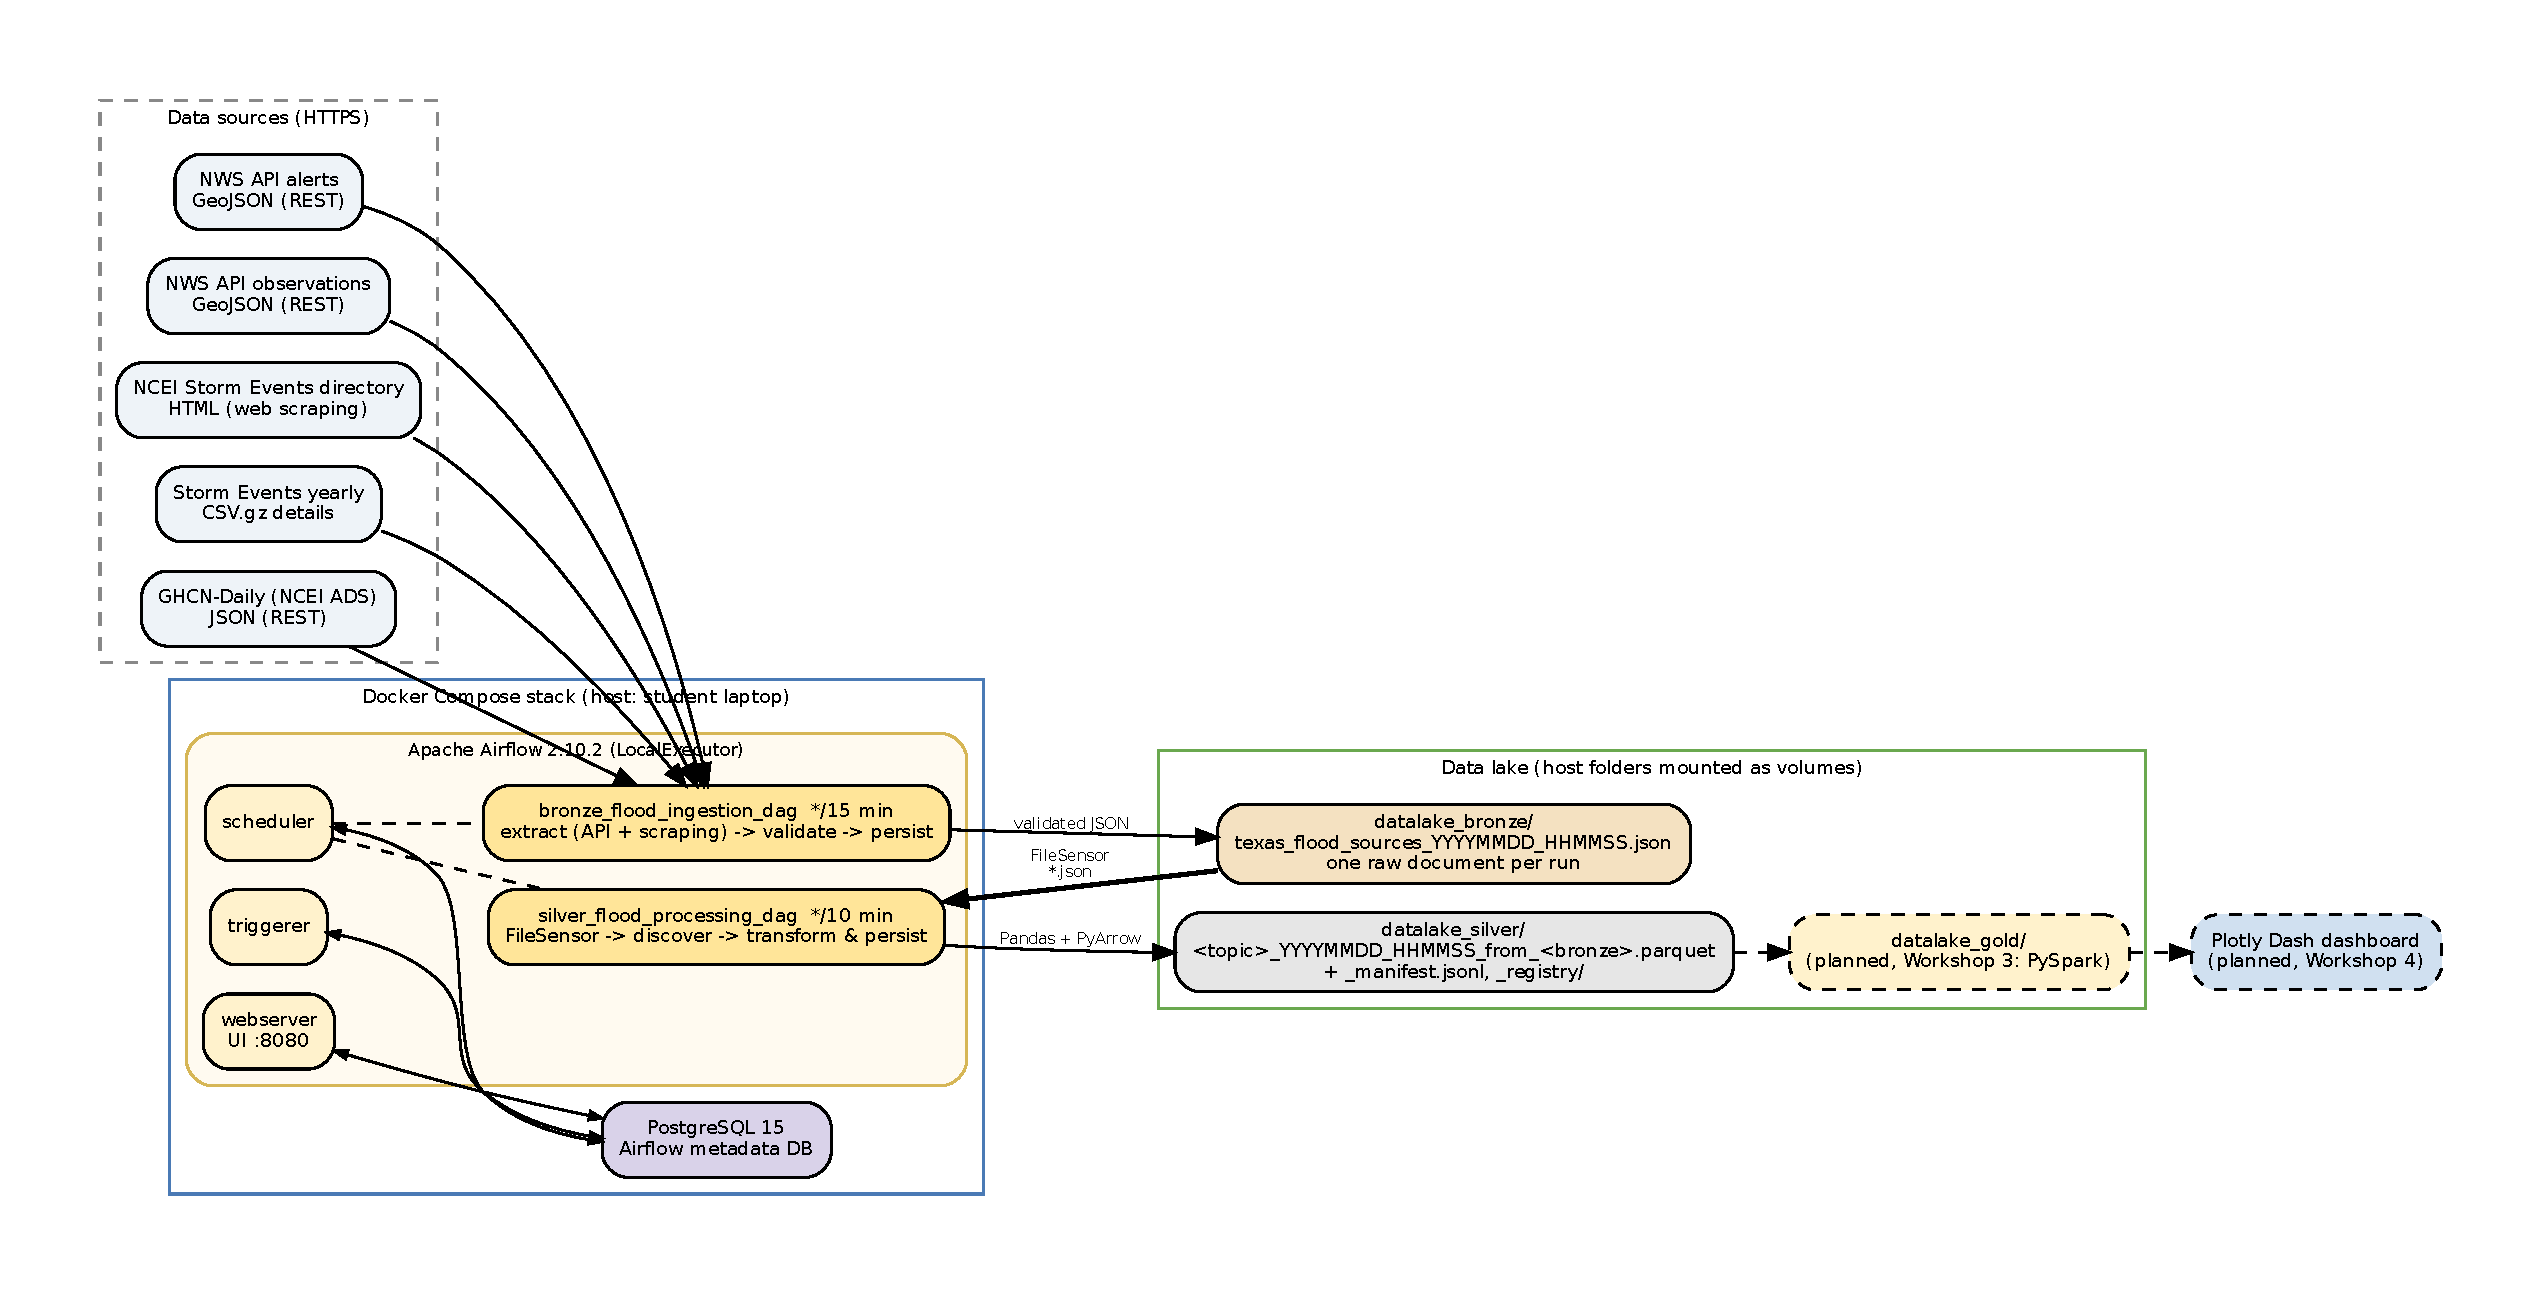
\includegraphics[width=\textwidth]{figures/architecture_w2.pdf}
\caption{System components, data flows and layer boundaries. Dashed elements are planned for Workshops 3--4.}\label{fig:arch}
\end{figure}

\subsection{Components}
\begin{longtable}{@{}p{2.5cm}p{3.1cm}p{2.4cm}p{3.1cm}p{3.5cm}@{}}
\caption{Purpose, technology, inputs, outputs and interactions of each component.}\label{tab:components}\\
\toprule Component & Purpose & Technology & Inputs $\rightarrow$ Outputs & Interactions\\\midrule\endhead
NWS API & Current observations and alerts & REST, GeoJSON & --- $\rightarrow$ JSON responses & Needs a \texttt{User-Agent} \citep{nws_api}; called by the Bronze DAG\\
NCEI Storm Events directory & Yearly files and their compile dates & HTML page (web scraping), CSV.gz files & --- $\rightarrow$ HTML, CSV & Scraped every run; files downloaded only when their watermark changes\\
NCEI Access Data Service & GHCN-Daily rainfall & REST, JSON & --- $\rightarrow$ JSON & One request per station (and per year in a backfill)\\
Airflow scheduler & Triggers DAG runs and runs tasks & Airflow 2.10.2, LocalExecutor & DAG files $\rightarrow$ task runs & Reads the mounted DAG folder; writes state to PostgreSQL\\
Airflow webserver & Monitoring, manual triggers, logs & Airflow UI, port 8080 & metadata DB $\rightarrow$ web UI & Reads and writes the metadata DB\\
Airflow triggerer & Runs deferrable operators & Airflow triggerer & deferred tasks $\rightarrow$ resumed tasks & Part of the required stack; ready for deferrable sensors\\
PostgreSQL 15 & Airflow metadata (runs, task states, XComs) & PostgreSQL & --- & Used by all Airflow services; flood data is not stored here yet\\
Bronze DAG & Extract, validate and persist raw data & TaskFlow API, \texttt{requests}, BeautifulSoup4 & sources $\rightarrow$ \texttt{datalake\_bronze/} & Atomic write; advances the Storm Events watermark only after the write\\
Bronze layer & Raw copy of every run & JSON & --- & Watched by the FileSensor\\
Silver DAG & Clean and type the data & FileSensor, Pandas, PyArrow & Bronze JSON $\rightarrow$ Parquet & Lineage in file names, columns, Parquet metadata and \texttt{\_manifest.jsonl}\\
Silver layer & Analysis-ready tables per topic & Apache Parquet (Snappy) & --- & Input of the Gold layer\\
Gold layer (planned) & Aggregates, Flood Risk Index & PySpark (Workshop 3) & Silver $\rightarrow$ Gold tables & Reads every file of a topic with one glob\\
Dashboard (planned) & Monitoring UI & Plotly Dash (Workshop 4) & Gold $\rightarrow$ web app & ---\\
\bottomrule
\end{longtable}

\subsection{Technology choices}
\begin{itemize}
  \item \textbf{Apache Airflow with the TaskFlow API} \citep{airflow_docs}: \texttt{@dag} and \texttt{@task} turn each step into a plain Python function, and the dependencies follow from the function calls. Payloads pass between tasks as XComs, which are stored in PostgreSQL. This is acceptable at our volume, where the largest XCom is the daily Storm Events delta of a few MB.
  \item \textbf{Web scraping with BeautifulSoup4}: the Storm Events data has no API. Its HTML directory is the only place that says which yearly files exist and when NOAA last re-compiled them (suffix \texttt{\_cYYYYMMDD}). Scraping it every run gives us the watermark that decides which files must be downloaded again.
  \item \textbf{Pandas for Silver} \citep{mckinney2010}: each batch fits easily in memory. The largest is the full Storm Events history, with 8{,}000 rows. Pandas also offers time-aware interpolation and is pinned by the Airflow constraints. Polars is installed in the image, but at this volume its speed would not change the result.
  \item \textbf{Parquet for Silver} \citep{parquet}: columnar, typed (UTC timestamps, lists for tokens and UGC codes) and compressed, with key-value metadata that we use for lineage. In Workshop~3, PySpark loads every Silver file of a topic with one glob.
  \item \textbf{Docker Compose} \citep{docker_compose}: one command reproduces the stack on every laptop. The \texttt{Dockerfile} installs \texttt{requirements-airflow.txt} with the Airflow~2.10.2 constraints, so our extra packages cannot change the versions Airflow depends on.
\end{itemize}

\subsection{File nomenclature}
\begin{itemize}
  \item \textbf{Bronze:} \texttt{datalake\_bronze/texas\_flood\_sources\_YYYYMMDD\_HHMMSS.json}. The source prefix is \texttt{texas\_flood\_sources}, because one document holds every source of a run. The timestamp is the UTC \emph{end of the run's data interval}, so re-running an interval overwrites the same file instead of adding a new one.
  \item \textbf{Silver:} \texttt{datalake\_silver/<topic>\_YYYYMMDD\_HHMMSS\_from\_<bronze stem>.parquet}, with \texttt{topic} $\in$ \{\texttt{nws\_observations}, \texttt{nws\_alerts}, \texttt{daily\_precipitation}, \texttt{flood\_events}\}. The timestamp is the UTC time of the processing run, as Workshop~3 requires, and the suffix names the Bronze file it came from.
  \item \textbf{Bookkeeping:} \texttt{datalake\_bronze/\_state/} stores the Storm Events watermarks. In Silver, \texttt{\_manifest.jsonl} records each Bronze file processed and what it produced, and \texttt{\_registry/} stores the keys and hashes already written.
\end{itemize}

% ===========================================================================
\section{Preprocessing Pipeline (Bronze $\rightarrow$ Silver)}
Every decision below answers a problem observed in the Workshop~1 samples. DQ~\#$n$ refers to Table~3 of the Workshop~1 report. The code is in \texttt{src/flood\_monitor/preprocessing.py} and \texttt{text.py}.

\subsection{Data-type normalization}
\begin{itemize}
  \item \textbf{Timestamps $\rightarrow$ \texttt{timestamp[UTC]}.}
  \begin{itemize}
    \item Storm Events times are local, with a two-digit year and the zone in a separate column (DQ~\#1). They are parsed with an explicit format and shifted by the offset in \texttt{CZ\_TIMEZONE}.
    \item NWS alert times carry \texttt{-05:00} or \texttt{-06:00} offsets (DQ~\#9) and are converted to UTC.
    \item GHCN values are local-day totals (DQ~\#5), so they are stored as dates, not instants.
  \end{itemize}
  \item \textbf{Measurements $\rightarrow$ \texttt{float64}; casualty counts $\rightarrow$ \texttt{int32}; severity $\rightarrow$ \texttt{int8}.} Damage strings with K/M/B suffixes (DQ~\#2) are parsed to USD.
  \item \textbf{Categories:} event type, message type, NWS severity, certainty, urgency, QC flags and GHCN flags become trimmed strings, with the sentinels \texttt{unknown}, \texttt{none} or \texttt{MISSING} instead of NULL. Parquet stores them with dictionary encoding.
  \item \textbf{Lists:} tokens, impact terms, UGC codes and alert references are stored as \texttt{list<string>}.
\end{itemize}

\subsection{Null handling}
\begin{longtable}{@{}p{3.4cm}p{3.2cm}p{7.9cm}@{}}
\caption{Null strategy per field (drop, impute, sentinel or flag).}\\
\toprule Field & Strategy & Justification\\\midrule\endhead
Keys and main timestamp & \textbf{Drop} row & A record without identity or time cannot be de-duplicated or placed on the timeline.\\
GHCN \texttt{PRCP} & \textbf{Drop} row & There is no value to analyse, and imputing rainfall would invent wet or dry days.\\
NWS \texttt{precipitationLastHour} & \textbf{NULL + flag} \texttt{precip\_missing} & In the Workshop~1 sample 98\% of observations had no value (\PrecipMissingPct\% in this workshop's runs), because only METAR reports carry rainfall (DQ~\#6). A missing hourly total is \emph{not} 0~mm, so severity also stays NULL. The first version filled these values with 0, and we reverted it.\\
NWS temperature & \textbf{Impute} by time interpolation (max.\ 2 steps) + flag & 5-minute series are smooth, so short gaps can be filled safely. Longer gaps stay NULL.\\
Alert \texttt{onset}, \texttt{ends} & \textbf{Impute} with \texttt{effective}, \texttt{expires} + flag & CAP semantics: an alert without onset starts when it becomes effective and lasts until it expires.\\
Storm Events damage & \textbf{NULL + flag} \texttt{damage\_missing} & An empty field means the damage is unknown, not zero (DQ~\#2).\\
Storm Events casualties & \textbf{Impute 0} (mode) & 0 is the overwhelming mode, and NOAA reports 0 when there were no casualties.\\
Coordinates & \textbf{NULL} (never 0,0) + \texttt{location\_known} & Records stay usable through the county or zone code.\\
Text and categories & \textbf{Sentinel} & \texttt{unknown}, \texttt{none} and \texttt{MISSING} keep group-bys and string operations simple.\\
\bottomrule
\end{longtable}

\subsection{Outlier detection and handling}
For floods, extreme rainfall \emph{is} the signal. Statistical outliers are therefore \textbf{flagged and kept}, and only physically impossible values are removed.
\begin{itemize}
  \item \textbf{Physical range (set to NULL + \texttt{out\_of\_range}):}
  \begin{itemize}
    \item hourly precipitation outside 0--250~mm (3~h: 0--500; 6~h: 0--750);
    \item daily PRCP outside 0--1000~mm;
    \item temperature outside $-40$ to 55~\textdegree C, and humidity outside 0--100\%;
    \item coordinates outside the Texas bounding box.
  \end{itemize}
  \item \textbf{IQR} \citep{tukey1977}: values above $Q_3 + 3\,\mathrm{IQR}$ are flagged on wet days per GHCN station (\texttt{is\_outlier\_iqr}) and on wet METAR hours (\texttt{is\_outlier\_precip}). $k=3$ is used because rainfall is strongly right-skewed. Damage is flagged above $Q_3 + 1.5\,\mathrm{IQR}$ on $\log_{10}$ USD. Quartiles are computed only with at least 10 values.
  \item \textbf{$Z$-score:} \texttt{prcp\_zscore} is computed on $\log(1+\text{PRCP})$ per station, and \texttt{is\_outlier\_z} marks $|z|>3$. The temperature $Z$-score is kept per station.
\end{itemize}
\gen{wettest.tex}

\subsection{Text preprocessing (NLP)}
Our topic contains free text in the Storm Events narratives and in the NWS alert headlines and descriptions. The pipeline in \texttt{text.py} is:
\begin{enumerate}
  \item lowercasing;
  \item URL removal;
  \item expansion of NWS abbreviations (\emph{hwy}, \emph{fm}, \emph{mph}, \emph{nws});
  \item unit normalization (``2.5in'' $\rightarrow$ ``2.5 inches'');
  \item removal of punctuation and of the ``\ldots'' separators of NWS products;
  \item whitespace tokenization;
  \item English stop-word removal, with an embedded list so the containers need no corpus download.
\end{enumerate}
Impact terms such as \emph{water rescue}, \emph{low water crossing} and \emph{stranded} are extracted as a list. The most frequent ones are: \TopTerms. Short categorical text (alert area, station description) keeps the lighter \texttt{normalize\_text}.

\subsection{De-duplication}
\begin{itemize}
  \item \textbf{Within a batch:} one row per natural key. The keys are \texttt{storm\_event\_id}, (\texttt{ghcn\_station\_id}, \texttt{obs\_date}), (\texttt{station\_id}, \texttt{ts\_utc}) and \texttt{alert\_id}.
  \item \textbf{Across batches:} each row has \texttt{event\_id} and a SHA-256 \texttt{record\_hash} of the raw record. \texttt{\_registry/<topic>\_keys.parquet} keeps the pairs already written. A known pair is skipped, and a known key with a new hash is written with \texttt{is\_update = true}. This is necessary because the incremental pulls overlap on purpose: 3~h for observations, 30 days for GHCN-Daily, and the recent alert window.
\end{itemize}

\subsection{Schema enforcement}
\texttt{preprocessing.SCHEMAS} defines the target schema of each topic: field name, Arrow type and whether the field is required. Before writing, rows missing a required field are dropped, columns are put in a fixed order, and the table is built with explicit types. Required fields are declared non-nullable. Six columns are common to all topics: \texttt{event\_id}, \texttt{source\_system}, \texttt{record\_hash}, \texttt{is\_update}, \texttt{bronze\_source\_file} and \texttt{processed\_at\_utc}.

% ===========================================================================
\section{Docker Stack}
\begin{table}[H]\centering\small
\caption{Services in \texttt{docker-compose.yml}.}
\begin{tabular}{@{}p{3cm}p{4.2cm}p{7cm}@{}}\toprule
Service & Image / command & Role\\\midrule
\texttt{postgres} & \texttt{postgres:15} & Airflow metadata DB; named volume; health check \texttt{pg\_isready}.\\
\texttt{airflow-init} & project image; creates folders, \texttt{db migrate}, admin user & One-shot initialization.\\
\texttt{airflow-webserver} & project image, \texttt{webserver} & UI at \url{http://localhost:8080}; health check on \texttt{/health}.\\
\texttt{airflow-scheduler} & project image, \texttt{scheduler} & Schedules and runs tasks (LocalExecutor).\\
\texttt{airflow-triggerer} & project image, \texttt{triggerer} & Runs deferrable operators.\\
\bottomrule\end{tabular}\end{table}

\paragraph{Image.} \texttt{FROM apache/airflow:2.10.2-python3.11}, then \texttt{pip install -r requirements-airflow.txt} (requests, beautifulsoup4, pandas, pyarrow, polars, pyyaml, python-dotenv) with the Airflow~2.10.2 constraints file.

\paragraph{Volumes.} \texttt{airflow/dags}, \texttt{airflow/logs}, \texttt{src}, \texttt{config}, \texttt{data}, \texttt{datalake\_bronze}, \texttt{datalake\_silver} and \texttt{datalake\_gold} are bind-mounted under \texttt{/opt/airflow}. All outputs stay on the host, and DAG edits are reloaded automatically.

\paragraph{Configuration and networking.} The services share the default Compose network and reach the database by its service name. The NWS contact, the webserver secret key and the admin password come from \texttt{.env} (\texttt{env\_file}). That file is git-ignored, and \texttt{.env.example} documents it. \texttt{AIRFLOW\_CONN\_FS\_DEFAULT} defines the filesystem connection of the FileSensor, and \texttt{PYTHONPATH=/opt/airflow/src} makes the \texttt{flood\_monitor} package importable from the DAGs.

\paragraph{Setup.}
\begin{lstlisting}
git clone https://github.com/natcastill/flood-monitoring-team2.git
cd flood-monitoring-team2
cp .env.example .env            # Windows: copy .env.example .env ; edit NWS_USER_AGENT
docker compose up -d --build    # http://localhost:8080  (admin / AIRFLOW_ADMIN_PASSWORD)
docker compose down             # data stays in the datalake_* folders
\end{lstlisting}

% ===========================================================================
\section{DAG Documentation}

\subsection{\texttt{bronze\_flood\_ingestion\_dag}}
\begin{itemize}
  \item \textbf{Schedule:} \texttt{*/15 * * * *}, the fastest cadence in the Workshop~1 contract (alerts every 15~min), with \texttt{catchup=False}, \texttt{max\_active\_runs=1} and 2 retries 2 minutes apart. Each source keeps its own contract cadence inside the DAG: observations hourly, GHCN-Daily and Storm Events details daily at 11:00~UTC. Parameters: \texttt{force\_all} pulls every source on demand, and \texttt{ghcnd\_backfill\_from} loads the GHCN-Daily history station $\times$ year.
  \item \textbf{Tasks:} \texttt{run\_context} $\rightarrow$ \texttt{extract\_nws\_alerts}, \texttt{extract\_nws\_observations}, \texttt{scrape\_storm\_events\_catalog} $\rightarrow$ \texttt{extract\_storm\_events\_details}, \texttt{extract\_ghcnd} $\rightarrow$ \texttt{validate\_bronze} $\rightarrow$ \texttt{persist\_bronze}.
  \begin{itemize}
    \item \emph{Validation} checks the structure of every payload, counts records missing required fields, and fails the run if the scraping found no files or no source returned records.
    \item \emph{Persistence} writes atomically (temporary file + rename) and only then advances the Storm Events watermark.
  \end{itemize}
  \item \textbf{Error handling and logging:} every task logs its counts. HTTP calls retry up to three times with exponential back-off on 429/5xx and on network errors. A failing station or GHCN request is logged and skipped, so the other sources still arrive.
\end{itemize}

\subsection{\texttt{silver\_flood\_processing\_dag}}
\begin{itemize}
  \item \textbf{Schedule:} every 10 minutes, \texttt{max\_active\_runs=1}.
  \item \textbf{\texttt{sense\_new\_bronze\_json}:} a \texttt{FileSensor} on \texttt{datalake\_bronze/texas\_flood\_sources\_*.json}.
  \begin{itemize}
    \item \texttt{poke\_interval=60}~s is how often it checks the folder. Bronze arrives every 15~min, so one check per minute is enough.
    \item \texttt{timeout=9}~min is how long it waits before giving up. It is shorter than the 10-minute schedule, so runs never overlap.
    \item \texttt{mode="reschedule"} frees the worker slot between checks (the first version used \texttt{poke}, which keeps it busy). \texttt{soft\_fail=True} marks the run \emph{skipped}, not \emph{failed}, when nothing arrives.
  \end{itemize}
  \item \textbf{\texttt{discover\_unprocessed\_bronze}:} lists the Bronze files that are not in \texttt{\_manifest.jsonl}. The first version compared file names with the Silver files, which reprocesses forever any Bronze file that produces no new rows.
  \item \textbf{\texttt{transform\_and\_persist\_silver}:} applies Section~3 to each topic of each Bronze file. It drops rows already in Silver, enforces the schema, and writes Parquet with the metadata keys \texttt{bronze\_source\_file}, \texttt{pipeline\_version} and \texttt{preprocessing\_stats}. It then updates the registry and the manifest.
\end{itemize}

\subsection{Idempotency}
\begin{itemize}
  \item \textbf{Bronze:} the file name depends only on the data interval, and the write is atomic.
  \item \textbf{Silver:} the manifest and the key/hash registry prevent reprocessing and duplicate rows.
\end{itemize}
The manifest of the real runs (below) shows Bronze files whose records were all skipped as \emph{already in Silver}, with no new Parquet written.
\lstinputlisting{generated/manifest.txt}

% ===========================================================================
\section{Results Evidence}

\subsection{Pipeline runs}
The corrected DAGs were run on 16--17 November 2026 against the live sources with Airflow (\texttt{airflow dags test}):
\begin{enumerate}
  \item the 23:30~UTC interval with \texttt{force\_all}: all sources, including the full Storm Events history 2010--2026;
  \item the 23:45~UTC interval with the normal cadence: alerts and the scraped catalog only;
  \item the 00:00~UTC interval: hourly observations, plus the GHCN-Daily history from 2010 (\texttt{ghcnd\_backfill\_from}).
\end{enumerate}
Silver ran after each of them.
\gen{bronze_inventory.tex}
\gen{silver_inventory.tex}

\subsection{Airflow UI}
\shot{airflow_dags_list.png}{Airflow UI (localhost:8080) listing the two DAGs.}{0.95}
\shot{bronze_ingestion_graph.png}{Graph view of a successful \texttt{bronze\_flood\_ingestion\_dag} run.}{0.95}
\shot{bronze_ingestion_grid.png}{Grid view with several successful runs of \texttt{bronze\_flood\_ingestion\_dag}.}{0.95}
\shot{silver_processing_graph.png}{Graph view of a successful \texttt{silver\_flood\_processing\_dag} run, starting with the FileSensor.}{0.95}
\shot{filesensor_log.png}{Log of \texttt{sense\_new\_bronze\_json} showing the FileSensor detecting Bronze files.}{0.95}

\subsection{Sample Bronze JSON}
\lstinputlisting{generated/bronze_sample.txt}

\subsection{Sample Silver Parquet content}
\gen{silver_sample.tex}
The largest damages are the Hurricane Harvey flash floods of August 2017. They show that the conversion of the ``10.00B'' damage strings and the local-time-to-UTC shift work on real records.

% ===========================================================================
\section{Challenges and Decisions}\label{sec:challenges}
\begin{itemize}
  \item \textbf{Repeated observations.} The first version requested the last 100 observations of each station every 30 minutes and de-duplicated only inside a file. Across its 11 Silver files, 4{,}884 of 5{,}500 observation rows (89\%) were repeats. We now request a bounded window (last hour + 3~h overlap) and skip rows already in Silver with the key/hash registry.
  \item \textbf{Missing is not zero.} The first version filled missing hourly rainfall with 0~mm, which contradicts Workshop~1 finding DQ~\#6. The value now stays NULL with a \texttt{precip\_missing} flag.
  \item \textbf{All four sources.} The first version stored only the Storm Events \emph{catalog}. Its watermark now drives a daily download of the changed yearly files (Texas flood rows), and GHCN-Daily was added with a 30-day overlap and an optional historical backfill.
  \item \textbf{Outliers that are the signal.} Removing statistical outliers would delete Harvey and other major floods. Outliers are therefore flagged with IQR and $Z$-score, and only impossible values are removed.
  \item \textbf{Dependencies.} Installing the whole project \texttt{requirements.txt} (Jupyter, Dash, a different pyarrow) into the Airflow image risked breaking Airflow. The image now installs a short \texttt{requirements-airflow.txt} with the official constraints.
  \item \textbf{Secrets and stray files.} The webserver secret key and admin password moved from \texttt{docker-compose.yml} to \texttt{.env}, a personal e-mail was removed from the code, and five empty files created by a mistyped shell command (\texttt{--role}, \texttt{--password}, \ldots) were deleted.
  \item \textbf{Empty responses are valid.} Texas often has no active flood alert. An empty payload passes validation, and Silver simply writes no file for that topic.
\end{itemize}

\bibliography{references}
\end{document}
